% *********************************************************************
% © 2021 Jeremy Sylvestre
%
% Permission is granted to copy, distribute and/or modify this document
% under the terms of the GNU Free Documentation License, Version 1.3 or
% any later version published by the Free Software Foundation; with no
% Invariant Sections, no Front-Cover Texts, and no Back-Cover Texts. A
% copy of the license is included in the appendix entitled “GNU Free
% Documentation License” that appears in the output document of this
% PreTeXt source code. All trademarks™ are the registered® marks of
% their respective owners.
%
% *********************************************************************

\newcommand*{\xmin}{-1}
\newcommand*{\xmax}{3}
\newcommand*{\ymin}{-0.5}
\newcommand*{\ymax}{6.5}

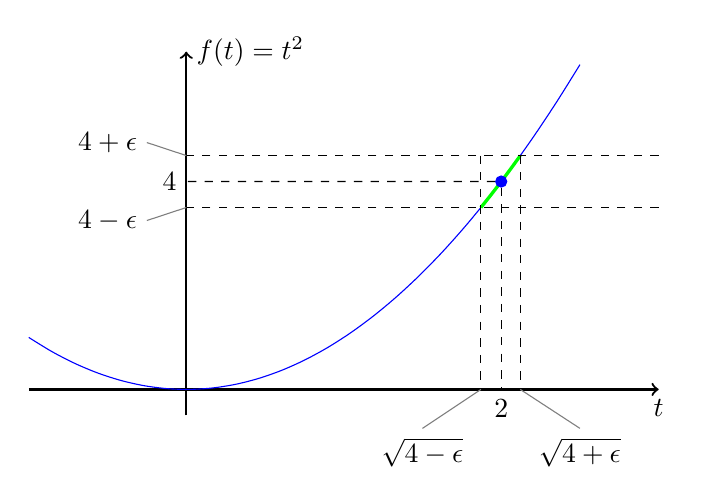
\begin{tikzpicture}
[
	closedpt/.style={circle,draw,fill,inner sep=0pt,minimum size=4pt},
	openpt/.style={circle,draw,inner sep=0pt,minimum size=4pt},
	yscale=0.66,xscale=2
]

	% axes
	\draw[->,thick] (\xmin,0) -- (\xmax,0) node[below] {$t$};
	\draw[->,thick] (0,\ymin) -- (0,\ymax) node[right] {$f(t) = t^2$};

	% graph
	\draw[blue, domain=-1:2.5, smooth] plot (\x,{\x * \x});

	\draw[very thick, green, domain=1.871:2.121, smooth] plot (\x,{\x * \x});

	\node[closedpt,blue] at (2,4) (p) {};

	\draw[dashed] (p) -- (2,0) node[below] {$2$};
	\draw[dashed] (p) -- (0,4) node[left] {$4$};
	\draw[dashed] (\xmax,4.5) -- (0,4.5);
	\draw[thin,gray] (0,4.5) -- (-0.25,4.75);
	\node[left] at (-0.25,4.75) {$4 + \epsilon$};
	\draw[dashed] (\xmax,3.5) -- (0,3.5);
	\draw[thin,gray] (0,3.5) -- (-0.25,3.25);
	\node[left] at (-0.25,3.25) {$4 - \epsilon$};

	\draw[dashed] (1.871,4.5) -- (1.871,0);
	\draw[dashed] (2.121,4.5) -- (2.121,0);

	\draw[thin,gray] (1.871,0) -- (1.5,-0.75);
	\node[below] at (1.5,-0.75) {$\sqrt{4 - \epsilon}$};
	\draw[thin,gray] (2.121,0) -- (2.5,-0.75);
	\node[below] at (2.5,-0.75) {$\sqrt{4 + \epsilon}$};

	% \foreach \x in {0.707, 1.225} {
	% 	\draw[dashed] (\x,0) -- (\x,1.5);
	% }

\end{tikzpicture}
